\documentclass[a4paper,titlepage]{article}
\usepackage{lingmacros}
\usepackage{tree-dvips}
\usepackage[italian]{babel}
\usepackage[utf8x]{inputenc}
\usepackage{amssymb}
\usepackage{graphicx}
%\usepackage{frontespizio}

\begin{document}
\tableofcontents

\newpage

\section{Introduzione}
In questo documento verranno presentati gli argomenti trattati per lo svolgimento del progetto di Sistemi con Vincoli, realizzato dagli studenti Rango Massimiliano, Segato Silvia e Tesselli Riccardo.\\Il progetto di interesse riguarda lo sviluppo di un risolutore automatico di CP-Nets sia acicliche che cicliche che adotta varie strategie di risoluzione.\\In questo documento verrà prima introdotto il problema iniziale, successivamente verranno presentate le fasi di lavoro svolte e descritte le nostre soluzioni al problema. Infine saranno visualizzati e analizzati i risultati ottenuti.

\section{Presentazione del problema}
Una CP-Net è una struttura che rappresenta reti di preferenze condizionali. Più formalmente una CP-Net sulle variabili $V = \{X_{1},\dots, X_{n}\}$ è un grafo orientato sui nodi $X_{1},\dots, X_{n}$, ogni nodo $X_{i} \in V$ è annotato con una tabella di preferenze condizionali $CPT(X_{i})$. Ogni tabella di preferenze condizionali $CPT(X_{i})$ associa un ordine totale $\succ^{i}_{\textbf{u}}$ con ogni instanziazione \textbf{u} dei genitori di $X_{i}$ detti $Pa(X_{i}) = U$. Una CP-Net si dice aciclica se il grafo che rappresenta non contiene cicli, altrimenti è detta ciclica.\\
Nel problema dato si vogliono individuare le soluzioni ottime, se esistono, di una CP-Net aciclica o ciclica, e individuare l'ordinamento parziale delle sue soluzioni. La ricerca delle soluzioni ottime è stata affrontata con diversi approcci. Il linguaggio di programmazione adottato è Java.\\Nella sessione successiva verranno presentate le varie fasi di lavoro.


\section{Fasi di sviluppo}

\subsection{Generazione Casuale di CPNets}
In primo luogo è stato sviluppato un codice per la generazione di CP-Nets casuali a partire da alcuni parametri scelti dall'utente, al fine di poter studiare il comportamento delle varie strategie di risoluzione al variare della struttura della CP-Net.\\
Il software genera una CP-Net in maniera casuale con numero di nodi e numero di archi fissati dall'utente. Per ogni nodo si generano le preferenze casualmente, supponendo che ogni nodo possa assumere due valori (negato o affermato), le preferenze generate garantiscono che il numero di condizioni per cui si preferisce il valore negato corrisponda al numero di condizioni per cui si preferisce il valore affermato, ovvero siano equamente distribuite.\\
Per la creazione l'algoritmo in primo luogo genera un grafo con il numero di nodi fissato dall'utente, ad ogni nodo viene assegnato un nome che corrisponde al numero cardinale del momento di creazione; successivamente estrae casualmente due nodi del grafo, uno di inizio e uno di fine, se dal nodo di inizio al nodo di fine non esiste già un arco orientato tra essi allora ne inserisce uno. Si continua a inserire archi fintanto che il numero di archi non corrisponde al parametro inserito dall'utente.\\
Come si può notare l'algoritmo di creazione di CP-Nets casuali può generare indistintamente reti cicliche o acicliche. Per distinguere la ciclicità di una CP-Net è stato sviluppato un algoritmo che controlla l'esistenza di cicli dato un grafo orientato.
\subsection{Studio dei paper} 

sicuri che questa serva????
\subsection{Implementazione algoritmi appresi}
\subsection{Strategie di Base}
I primi algoritmi implementati per trovare le soluzioni ottime di CP-Nets sono quelli appresi e messi in pratica a lezione.

\subsubsection{Algoritmo per CP-Nets acicliche: Sweep Forward}
L'algoritmo implementato per trovare l'unica soluzione ottima di una CP-Net aciclica è denominato Sweep Forward e consiste nel seguire le dipendenze del grafo. In particolare, consiste nell'assegnare il valore ``preferito'' ad ogni variabile nel contesto degli assegnamenti fatti per i genitori.

\subsubsection{Algoritmo per CP-Nets cicliche}
Data una CP-Net ciclica, per trovare le sue soluzioni ottime si deve ricavare un insieme di vincoli $P$, tale che le soluzioni di $P$ coincidono con l'insieme delle soluzioni ottime della CP-Net. Tale insieme $P$ lo si riesce a  trovare in tempo polinomiale.

\subsubsection{Implementazione}
Il metodo che si occupa di trovare le soluzioni ottime della CP-Net generata è il seguente
\\
\\
\centerline{\texttt{public List<Assignment> getOptimalSolution(Inference strategy, boolean findAll)}}
\\

Tale metodo adotta le due strategie descritte sopra in base alla ciclicità della CP-Net data.
Ogni soluzione ottima della CP-Net è stata implementata come assegnamento (oggetto di tipo \texttt{Assignment}); un assegnamento è una mappa $\langle$variabile, valore$\rangle$.
L'algoritmo Sweep Forward per CP-Nets acicliche è stato implementato come metodo della classe \texttt{CPNet}:\\
\\
\centerline{\texttt{public Assignment solveAcyclicCPNet(Assignment result, List<Variable> vars)}}
\\

La soluzione ottima in questo caso corrisponde alla variabile \texttt{result}.
Per ciascuna variabile indipendente, viene settato in \texttt{result} il relativo assegnamento con il valore preferito.
Dopo ciò si controllano le variabili non indipendenti, precedentemente inserite in una lista; per ciascuna di queste, si controlla se i suoi genitori hanno già un valore assegnato in \texttt{result}. Se così è, allora in base all'assegnamento dei genitori si sceglie il valore preferito per la variabile in esame e lo si usa per settare l'assegnamento di quest'ultima in \texttt{result}. Fatto ciò si toglie la variabile dalla lista e si ricomincia l'analisi con le rimanenti variabili. Qualora la variabile in esame non avesse ancora una configurazione completa per tutti i suoi genitori, la si lascia nella lista e si prosegue con la successiva.
\\
Al fine di poter attuare la strategia di risoluzione per CP-Nets cicliche, il primo passo da effettuare è la conversione da CP-Net a CSP. 
\\
I CSPs che si vengono a creare consistono di variabili, ciascuna delle quali ha come dominio \{0, 1\}, e un insieme di vincoli.
A livello implementativo, ciò corrisponde alla creazione della classe \texttt{CSP} e \texttt{Variable}, nonché dell'interfaccia \texttt{Constraint}.
 
I vincoli rispettano il seguente pattern:
\\
\centerline{ipotesi $\rightarrow$ tesi}

Tesi e ipotesi si compongono di assegnamenti. La tesi contiene l'assegnamento di un unica variabile, l'ipotesi contiene disgiunzioni di congiunzioni di assegnamenti (ad esempio, la seguente può essere una ipotesi: $( (A=1 \land B=1) \lor (A=0 \land B=0))$ ). 

Tale tipo di vincolo è stato implementato con la creazione della classe \texttt{Implies}, che implementa \texttt{Constraint}.


La classe \texttt{CPNetCSP} si occupa di creare un CSP di questo tipo, dopo aver opportunamente creato le variabili a partire dai vertici del grafo, tramite il metodo
\\
\centerline{\texttt{private List<Variable> generateVariables()}}
\\
e i vincoli a partire dalle preferenze,tramite il metodo
\\
\centerline{\texttt{private List<Implies> generateConstraints(List<Variable> variables)}}
\\

Per trovare le soluzioni del CSP così creato è stata utilizzata la classe astratta\texttt{SolvingStrategy} e la sua sottoclasse \texttt{BacktrakingStrategy}. Come dice il nome stesso, tale classe si occupa di implementare la strategia di risoluzione di un CSP attraverso la ricerca con Backtraking. L'algoritmo implementato è in grado di trovare tutte le soluzioni ottime del CSP datogli in input. Tuttavia, l'utente finale può scegliere se lasciare che l'algoritmo trovi tutte le soluzioni o si fermi alla prima soluzione.

L'utente è anche in grado di scegliere se eseguire l'algoritmo di Backtraking ``di base'', o se con Forward Checking o con propagazione di vincoli (AC3). Per permettere ciò, si è utilizzata una sottoclasse di \texttt{BacktrakingStrategy}, denominata \texttt{ImprovedBacktrakingStrategy}, e una nuova classe, \texttt{AC3Strategy}, che si occupa della propagazione di vincoli.



\subsection{Creazione dell'ordinamento parziale delle soluzioni}

Per poter ottenere l'ordinamento parziale delle soluzioni, occorre eseguire il metodo
\\
\centerline{\texttt{public boolean generatePartialOrderSolution()}}
\\

Tale metodo si occupa di creare un oggetto \texttt{PartialOrderSolutionGraph}, che rappresenta il grafo delle soluzioni. In particolare,  l'oggetto contiene una lista di oggetti \texttt{Solution}, ognuno dei quali contiene, oltre al valore della soluzione stessa che, per brevità, è una stringa (ad esempio, in una CPnet che ha, nell'ordine, A, B, C come variabili, un oggetto \texttt{Solution} ha come valore ``111'', che è da intendersi come l'equivalente di {A=1, B=1, C=1}), anche la lista dei valori di quelle soluzioni che sono sotto di lei nell'ordinamento (da ora in avanti queste verranno chiamate ``sottoliste'').
Per costruire il grafo vero e proprio, viene richiamato il metodo 
\\
\centerline{\texttt{public void setPartialOrderSolutions()}}
\\

Esso si occupa di settare le sottoliste di ciascuna 
soluzione. In questo modo, il grafo viene memorizzato come una lista di adiacenze.

\subsection{Implementazione soluzione con local search}


\section{Risultati e statistiche}

\section{Consultivo finale}

\section{Appendice: Istruzioni d'uso}
Il software viene fornito sotto forma di JAR eseguibile. Per lanciare l'esecuzione bisogna eseguire da console il comando
\begin{verbatim}
java -jar CPNets.jar <strategy> <nNodi> <nArchi> <findAll>
\end{verbatim}
dove \texttt{<strategy>}, \texttt{<nNodi>}, \texttt{<nArchi>}, \texttt{<findAll>} sono i parametri.\\
Il parametro \texttt{<strategy>} definisce con quale strategia si vogliono individuare le soluzioni della CP-Net, i valori ammessi sono:
\begin{itemize}
\item  \texttt{ls} : Local Search;
\item  \texttt{fc} : Backtracking + Forward Checking;
\item  \texttt{ac3} : Backtracking + consistenza d'arco;
\item  \texttt{none} : Backtracking.
\end{itemize}
I parametri \texttt{<nNodi>}, \texttt{<nArchi>} definiscono rispettivamente il numero di nodi e archi della CP-Net da generare.\\
Infine il parametro \texttt{<findAll>} è un parametro booleano, se è \texttt{true} allora l'algoritmo di risoluzione individuerà l'ordinamento parziale di tutte le soluzioni del problema, se altrimenti è \texttt{false} verrà individuata solo quella ottima. Questo parametro viene utilizzato solo nel caso di strategie che richiedono backtracking, non si applica alla strategia Local Search.\\
Una volta lanciato il comando comparirà una interfaccia grafica come visualizzato in figura \ref{fig:1}.\\
\begin{figure}
\centering
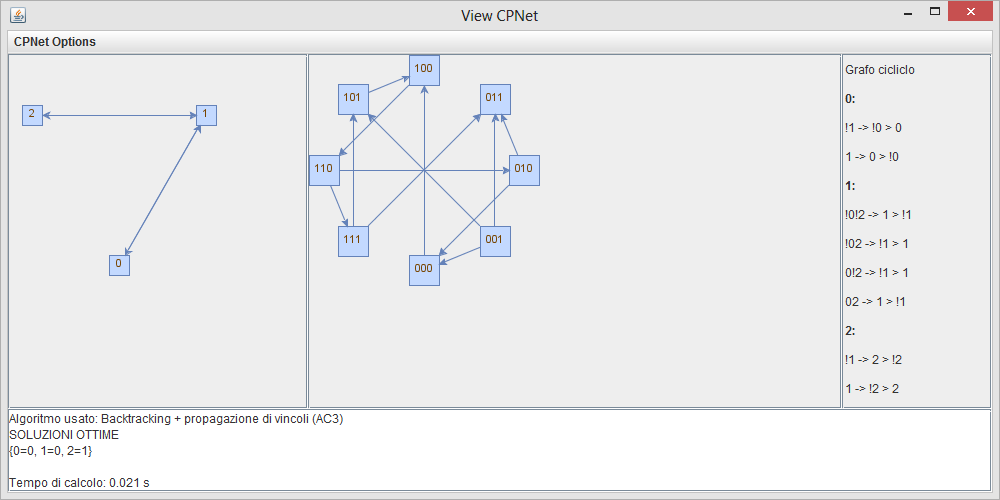
\includegraphics[scale=0.5]{../img/screen.png}
\caption{Esempio di schermata}\label{fig:1}
\end{figure}
Nel riquadro a sinistra viene visualizzata la struttura della CP-Net; nel pannello a destra viene mostrata la ciclicità della rete e le tabelle di preferenze condizionali di ogni variabile. Si assume che data una variabile $X$ i valori per tale variabile sono $x$ per i valori affermati e $!x$ per i valori negati.\\
Nel pannello centrale viene visualizzato il grafo che rappresenta l'ordinamento parziale di tutte le soluzioni della CP-Net. Ogni nodo del grafo rappresenta una instanziazione dei valori delle variabili. Una instaziazione è intesa come un assegnamento ordinato di valori 0, per valori negati, e 1 per valori affermati. L'ordine di assegnazione è determinato in senso crescente, ovvero il primo valore si riferisce alla variabile 0 e così via fino all'ultima variabile. Se una instanziazione $A$ è migliore di una instanziazione $B$ allora compare un arco orientato da $A$ a $B$ nel grafo. Per visualizzare l'ordinamento parziale delle soluzioni è necessario che il parametro \texttt{<findAll>} sia \texttt{true} e cliccare sul menù a tendina in alto a sinistra.\\
Nel pannello inferiore viene visualizzato un riassunto della strategia utilizzata, della soluzione ottima individuata e del tempo di calcolo richiesto.

\end{document}